\section{Модальный регулятор}

Рассмотрим систему $\dot{x} = Ax + Bu$, где 
\begin{equation}
    \begin{gathered}
        A = \begin{bmatrix}
            4 & 6 & 4 \\
            -4 & -6 & -6 \\
            4 & 4 & 4
        \end{bmatrix}, \quad
        B = \begin{bmatrix}
            4 \\
            -1 \\
            1
        \end{bmatrix}, \quad
        \begin{cases}
            \sigma_1 &= \{-1, -1, -1\} \\
            \sigma_2 &= \{-2, -2, -2\} \\
            \sigma_3 &= \{-1, -10, -100\} \\
            \sigma_4 &= \{-2, -20, -200\} \\
            \sigma_5 &= \{-1, -1 - 3i, -1 + 3i\} \\
            \sigma_6 &= \{-2, -2 - 6i, -2 + 6i\}
        \end{cases}
    \end{gathered}
\end{equation}

\subsection{Управляемость системы}

\subsubsection{Управляемость собственных значений}
Найдем спектр матрицы $A$:
\begin{equation}
    \sigma(A) = \{-2, 2-2j, 2+2j\}
\end{equation}

Для каждого собственного значения найдем матрицу Хаутуса $H_i = \begin{bmatrix} A - \lambda_i I & B \end{bmatrix}$ и определим ее ранг:
\begin{enumerate}
    \item $\lambda_1 = -2$: $H_1 = \begin{bmatrix}
        6 & 6 & 4 & 4\\
        -4 & -4 & -6 & -1 \\
        4 & 4 & 6 & 1
    \end{bmatrix}$, $\text{rank}(H_1) = 2$, собственное значение неуправляемо.
    \item $\lambda_2 = 2-2j$: $H_2 = \begin{bmatrix}
        2+2j & 6 & 4 & 4\\
        -4 & -4+2j & -6 & -1 \\
        4 & 4 & 6+2j & 1
    \end{bmatrix}$, $\text{rank}(H_2) = 3$, собственное значение управляемо.
    \item $\lambda_3 = 2+2j$: $H_3 = \begin{bmatrix}
        2+2j & 6 & 4 & 4\\
        -4 & -4+2j & -6 & -1 \\
        4 & 4 & 6+2j & 1
    \end{bmatrix}$, $\text{rank}(H_3) = 3$, собственное значение управляемо.
\end{enumerate}

Собственное число $\lambda_1$ является \textbf{неуправляемым}. Следовательно, согласно критерию Хаутуса, система \textbf{не является полностью управляемой}.  
Однако система будет \textbf{стабилизируемой}, так как все \textbf{неустойчивые собственные числа} (если таковые имеются) оказываются \textbf{управляемыми}.

\subsection{Достижимые спектры}
Не все спектры могут быть использованы в качестве достижимых для матрицы замкнутой системы $(A + BK)$, так как система \textbf{не является полностью управляемой}. Это ограничение связано с неуправляемым собственным числом $\lambda_3 = -2$, которое \textbf{нельзя изменить с помощью регулятора}. Следовательно, $\lambda_3$ обязательно останется одним из собственных чисел матрицы $(A + BK)$ после замыкания системы. После отбора доступных спектров остаются следующие, которые уже являются достижимыми:

\[
\sigma_2 = \{-2, -2, -2\}, \quad
\sigma_4 = \{-2, -20, -200\}, \quad
\sigma_6 = \{-2, -2 - 6i, -2 + 6i\}.
\]

\subsubsection{Первый спектр}
Задан желаемый спектр замкнутой системы:
\[
\sigma_1 = \{-2, -2, -2\}.
\]

Для нахождения матрицы регулятора $K$, которая обеспечивает данный спектр, воспользуемся следующей системой уравнений:
\[
\begin{cases}
AP - PG = BY, \\
K = -Y P^{-1},
\end{cases}
\]
где:
\begin{itemize}
    \item $P$ — матрица преобразования,
    \item $G$ — матрица с желаемым спектром,
    \item $Y$ — вспомогательная матрица.
\end{itemize}

Перед синтезом регулятора убедимся, что выполняются следующие условия:
\begin{enumerate}
    \item Спектры матриц $A$ и $G$ не пересекаются: $\sigma(A) \cap \sigma(G) = \emptyset$.
    \item Пара $(A, B)$ является управляемой (или хотя бы стабилизируемой).
    \item Пара $(Y, G)$ является наблюдаемой.
\end{enumerate}

Матрицы $G$ и $Y$ выбираются следующим образом:
\begin{itemize}
    \item $G \in \mathbb{R}^{n \times n}$ — матрица с желаемым спектром $\sigma(G)$.
    \item $Y \in \mathbb{R}^{m \times n}$ — матрица, обеспечивающая наблюдаемость пары $(Y, G)$.
\end{itemize}

Затем решаем уравнение Сильвестра $AP - PG = BY$ для нахождения $P$ и вычисляем регулятор $K = -Y P^{-1}$.

В нашем случае пара $(A, B)$ является \textbf{стабилизируемой}, но не полностью управляемой. Это означает, что решение может быть не единственным или вырожденным. Однако, выбрав $G$ и $Y$ следующим образом:
\[
G = \begin{bmatrix}
-2 & 1 & 0 \\
0 & -2 & 1 \\
0 & 0 & -2
\end{bmatrix}, \quad
Y = \begin{bmatrix}
1 & 0 & 1
\end{bmatrix},
\]
мы обеспечиваем выполнение всех необходимых условий.

После вычислений получаем коэффициенты регулятора:
\[
K = \begin{bmatrix}
-1.94 & -1.94 & -1.94
\end{bmatrix}.
\]
\newpage
Собственные числа матрицы замкнутой системы $(A + BK)$ :
\[
\lambda_{1,2,3} \approx -2,
\]
что соответствует заданному спектру $\sigma_1$. Это подтверждает корректность синтеза регулятора.

\begin{figure}[H]
    \centering
    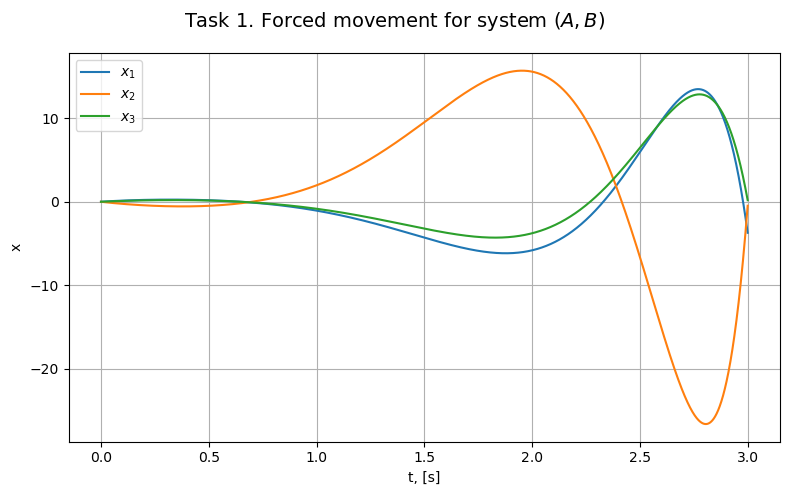
\includegraphics[width=0.8\textwidth]{../../plots/task_1_1.png}
    \caption{Состояние системы}
    \label{fig:task_1_state_system_1}
\end{figure}

\begin{figure}[H]
    \centering
    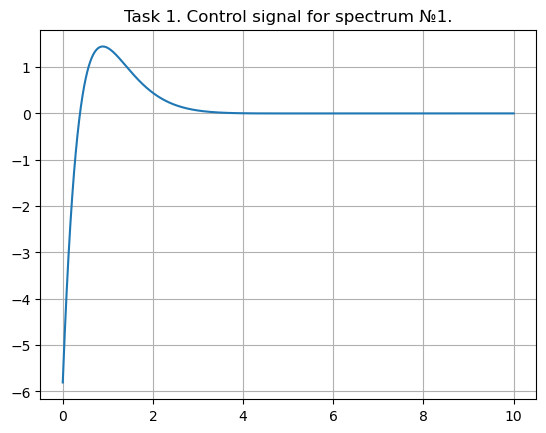
\includegraphics[width=0.8\textwidth]{../../plots/task_1_2.png}
    \caption{Сигнал управления}
    \label{fig:task_1_control_signal_1}
\end{figure}

\subsubsection{Второй спектр}

Рассмотрим второй желаемый спектр замкнутой системы:
\[
\sigma_2 = \{-2, -20, -200\}.
\]

Для нахождения матрицы регулятора $K$ воспользуемся следующей системой уравнений:
\[
\begin{cases}
AP - PG = BY, \\
K = -Y P^{-1},
\end{cases}
\]
где:
\begin{itemize}
    \item $P$ — матрица преобразования,
    \item $G$ — матрица с желаемым спектром,
    \item $Y$ — вспомогательная матрица.
\end{itemize}

Для решения системы выберем матрицы $G$ и $Y$ следующим образом:
\[
G = \begin{bmatrix}
-2 & 0 & 0 \\
0 & -20 & 0 \\
0 & 0 & -200
\end{bmatrix}, \quad
Y = \begin{bmatrix}
0 & 1 & 1
\end{bmatrix}.
\]

После выполнения вычислений получаем коэффициенты регулятора:
\[
K = \begin{bmatrix}
26.08 & 164.16 & -164.16
\end{bmatrix}.
\]

Собственные числа матрицы замкнутой системы $(A + BK)$:
\[
\lambda_1 = -2, \quad \lambda_2 = -20, \quad \lambda_3 = -200.
\]

Эти значения соответствуют заданному спектру $\sigma_2$, что подтверждает корректность синтеза регулятора.

\begin{figure}[H]
    \centering
    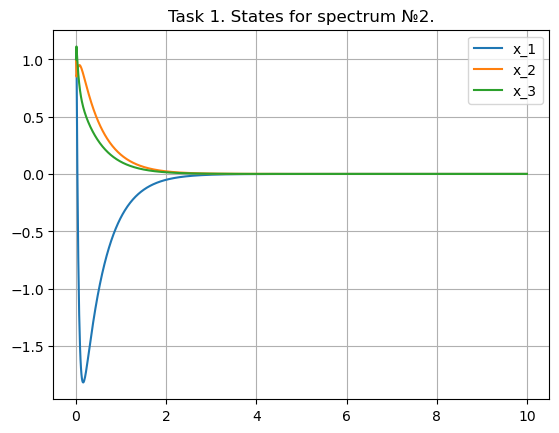
\includegraphics[width=0.8\textwidth]{../../plots/task_1_3.png}
    \caption{Состояние системы}
    \label{fig:task_1_state_system_2}
\end{figure}

\begin{figure}[H]
    \centering
    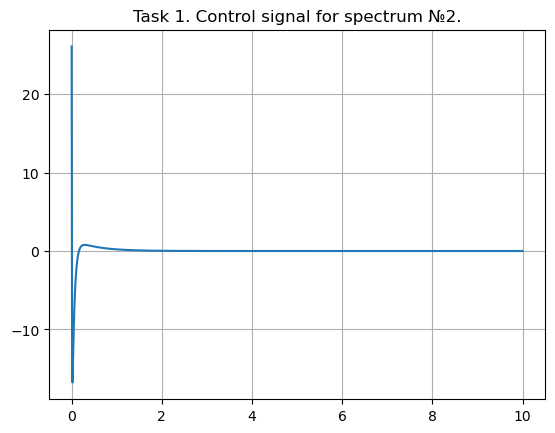
\includegraphics[width=0.8\textwidth]{../../plots/task_1_4.png}
    \caption{Сигнал управления}
    \label{fig:task_1_control_signal_2}
\end{figure}


\subsubsection{Третий спектр}

Рассмотрим третий желаемый спектр замкнутой системы:
\[
\sigma_2 = \{-2, -2-6j, -2+6j\}.
\]

Для нахождения матрицы регулятора $K$ воспользуемся следующей системой уравнений:
\[
\begin{cases}
AP - PG = BY, \\
K = -Y P^{-1},
\end{cases}
\]
где:
\begin{itemize}
    \item $P$ — матрица преобразования,
    \item $G$ — матрица с желаемым спектром,
    \item $Y$ — вспомогательная матрица.
\end{itemize}

Для решения системы выберем матрицы $G$ и $Y$ следующим образом:
\[
G = \begin{bmatrix}
-2 & 0 & 0 \\
0 & -2 & 6 \\
0 & -6 & -2
\end{bmatrix}, \quad
Y = \begin{bmatrix}
0 & 1 & 1
\end{bmatrix}.
\]

После выполнения вычислений получаем коэффициенты регулятора:
\[
K = \begin{bmatrix}
-1.28 & 1.44 & -1.44
\end{bmatrix}.
\]

Собственные числа матрицы замкнутой системы $(A + BK)$:
\[
\lambda_1 = -2, \quad \lambda_2 = -2-6j, \quad \lambda_3 = -2+6j.
\]

Эти значения соответствуют заданному спектру $\sigma_3$, что подтверждает корректность синтеза регулятора.

\begin{figure}[H]
    \centering
    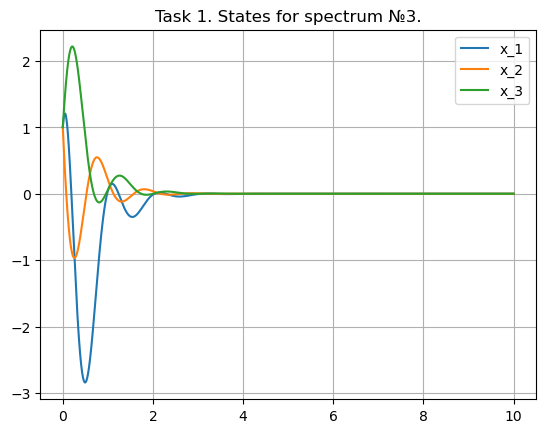
\includegraphics[width=0.8\textwidth]{../../plots/task_1_5.png}
    \caption{Состояние системы}
    \label{fig:task_1_state_system_3}
\end{figure}

\begin{figure}[H]
    \centering
    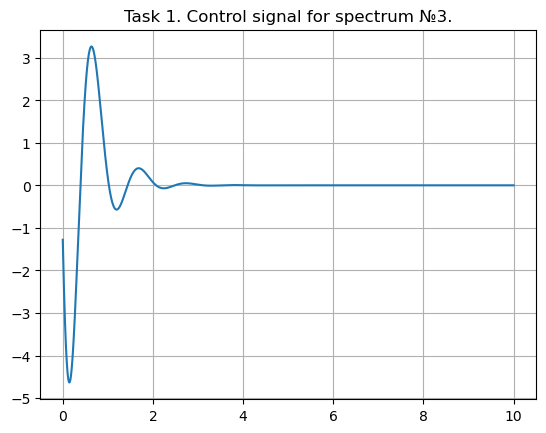
\includegraphics[width=0.8\textwidth]{../../plots/task_1_6.png}
    \caption{Сигнал управления}
    \label{fig:task_1_control_signal_3}
\end{figure}


\subsection{Сравнение выбора спектра для синтеза регулятора}

\subsubsection{Первый спектр}
Мы выбрали относительно небольшие устойчивые моды. В результате регулятор корректировал систему плавно, с минимальным перерегулированием. Это обеспечило стабильное и предсказуемое поведение системы.

\subsubsection{Второй спектр}
Для ускорения процесса управления мы значительно увеличили моды. Это привело к агрессивному управлению, которое быстро привело систему в нулевую позицию. Однако в реальных условиях такое управление может быть неприменимо из-за физических ограничений

\subsubsection{Третий спектр}
В спектр были включены комплексно-сопряжённые моды. Это привело к сходимости системы с небольшими колебаниями, но в целом плавно и с умеренным перерегулированием. Вещественная часть этих мод не слишком велика, что обеспечивает баланс между скоростью и стабильностью.


\subsection{Вывод}
Проведённое исследование системы показало, что даже \textbf{стабилизируемая система} (которая не обязательно является полностью управляемой) позволяет реализовать управление с различными характеристиками сходимости. Мы успешно синтезировали \textbf{модальный регулятор}, используя уравнение Сильвестра. Совпадение желаемых спектров со спектром матрицы замкнутой системы $(A + BK)$ подтверждает корректность выполненного синтеза.